\documentclass[12pt]{article}
\usepackage{amssymb}
\usepackage{amsthm}
\usepackage{amsmath}
\usepackage{float}
\usepackage{graphicx}
\usepackage{breqn}
\usepackage[margin=1in]{geometry}
\newcommand{\parder}[2]{\frac{\partial}{\partial{#2}}#1}
\newcommand{\parderpow}[3]{\frac{\partial^{#3}}{\partial{#2}^{#3}}#1}
\newcommand{\parderplace}[2]{\frac{\partial{#1}}{\partial{#2}}}
\newcommand{\parderpowplace}[3]{\frac{\partial^{#3}{#1}}{\partial{#2}^{#3}}}
\newcommand{\Exp}{\mathrm{Exp}}
\newcommand{\bra}[1]{\langle #1}
\newcommand{\ket}[1]{\lvert #1 \rangle}
\newcommand{\highlight}[2]{\colorbox{#2}{$\displaystyle #1$}}
\renewcommand{\thesubsection}{(\alph{subsection})}

\usepackage{minted}
\usepackage[caption=false]{subfig}

\begin{document}
\title{Ph 121a Assignment 4: Molecular Dynamics}
\author{Nicholas Meyer}

\maketitle

\section{Approach}

Here, a neutral noble gas in two dimensions on a torus was modeled using the
Lennard-Jones potential for each pairwise interaction between particles:

\begin{align}
  U_{LJ}(r) &= \epsilon \left[\left(\frac{r_{\text{min}}}{r}\right)^{12}
  - 2\left(\frac{r_{\text{min}}}{r}\right)^6\right] \\
  m\vec{a} &= -\parderplace{U(r)}{r}\hat{r}
\end{align}

A Langevin-Verlet integrator was used to evolve the particle positions through
time using the following update rule:

\begin{align}
  \vec{r}(t + h)
  &= A\vec{r}(t) + B\vec{r}(t - h) + C\vec{a}(t)
  + D(\vec{W}(t) + \vec{W}(t - h))
\end{align}

where $A, B, C, D$ are functions of the step size, parameter $\alpha$, and
the temperature (as calculated in the assignment document), and
$\vec{W}(t)$ is a tuple of standard normally distributed random variables.

\section{Implementation}

The routines for calculating the forces between particles and updating the
positions through the Langevin-Verlet integrator are in C++.
Control of the running simulations and plotting are done in python, using
\mintinline{python}/ctypes/ to interface with the C++ code.

\subsection{Normally distributed random values}

To obtain normally distributed random variables, the Box-Muller transform
was applied to uniformly distributed random numbers on the interval $[0, 1)$:
($u_i$ are random variables from a uniform distribution from $0$ to $1$,
$n_i$ are normally distributed with a mean of $0$ and a standard deviation
of $1$)

\begin{align}
  n_1 &= \sqrt{ -2\log{u_1}} * \cos{(2\pi u_2)} \\
  n_2 &= \sqrt{ -2\log{u_1}} * \sin{(2\pi u_2)}
\end{align}

\subsection{Use of double precision instead of single floats}

When single precision floating point numbers were used for particle positions
and simulation parameters, particles would accelerate toward the bottom left
corner of the screen. The drift was most noticeable for temperatures close to
zero. This was likely due to the accumulation of rounding error (which was
for some reason consistently biased toward rounding down) over many
iterations.

This behavior was fixed by switching to double precision floats.

\section{Running the suite}

First, it is necessary to build the dynamic library by running

\begin{minted}{bash}
make molec.so
\end{minted}

Then, the visualizer can be run from the command line, i.e.

\begin{minted}{bash}
python visualizer.py 1.0 movie 1000
\end{minted}

to make a movie with 1000 frames of the system starting at a solid and
evolving when the temperature is suddenly set to one, or

\begin{minted}{bash}
python visualizer.py 5.0
\end{minted}

to view the animation for $T = 5$.

\section{Plots}

The simulation torus was defined to have a period of $30$ in both the $x$ and
$y$ directions.

Initial conditions for 100 points in a solid configuration
were obtained by randomly initializing
molecules (at a distance at least $1$ from one another) and then gradually
lowering the temperature to zero. These values are stored in a local
variable (\mintinline{python}/initial_data/)in the
\mintinline{python}/if __name__=="__main__"/ segment of \texttt{visualize.py}.

Starting from these initial conditions, evolutions were run at different
temperatures to simulate a transition to different states. Note that the
units on the temperature are somewhat arbitrary since the Boltzmann constant
$k_B$ has been set to $1$, as have most physical parameters of the system.

\subsection{Solid}

The solid simulation was run by evolving from the initial conditions with
a temperature of zero.

To view as an animation, run

\begin{minted}{bash}
python visual
\end{minted}

The frames for the animated gif (see github) were created using the command:

\begin{minted}{bash}
python visualize.py 0 movie temp0 1000
\end{minted}

\begin{figure}[H]
  \subfloat{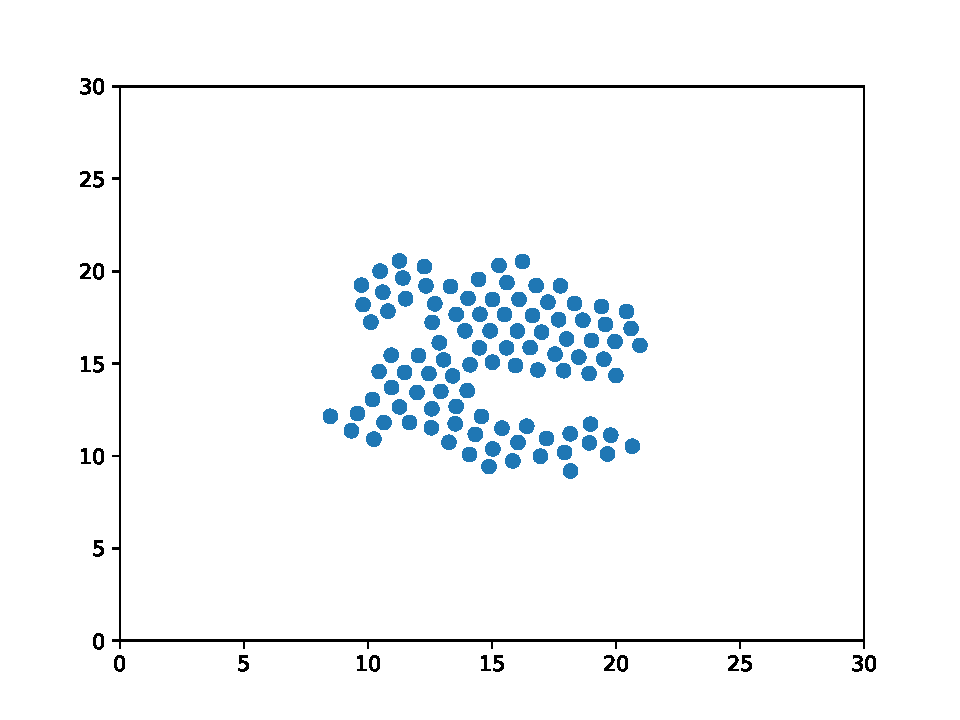
\includegraphics[width=0.5\linewidth]{writeup_plots/T0_start.pdf}}
  \subfloat{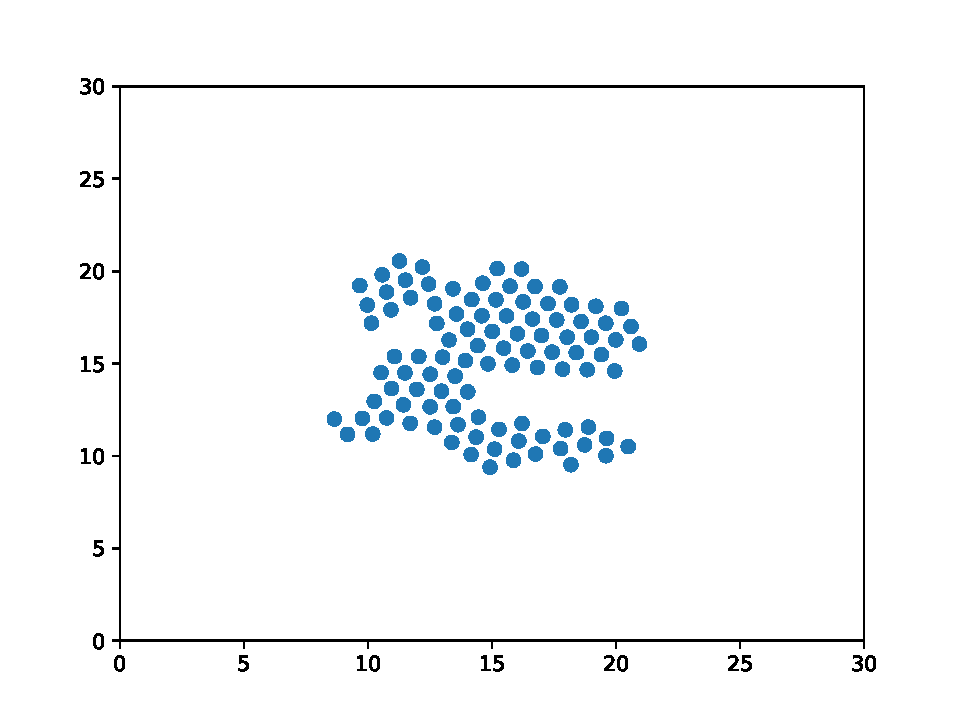
\includegraphics[width=0.5\linewidth]{writeup_plots/T0_end.pdf}}
  \caption{(Left to right) starting and ending configuration after $10000$
    timesteps of $h = 1e-3$.}
\end{figure}

\subsection{Liquid}

The liquid simulation was run by evolving from the initial conditions with a
temperature of $10$. If this system is evolved long enough, the liquid
eventually vaporizes.

To view as an animation, run

\begin{minted}{bash}
python visualize.py 10
\end{minted}

The frames for the animated gif (see github) were created using the command:

\begin{minted}{bash}
python visualize.py 10 movie temp10 1000
\end{minted}

\begin{figure}[H]
  \subfloat{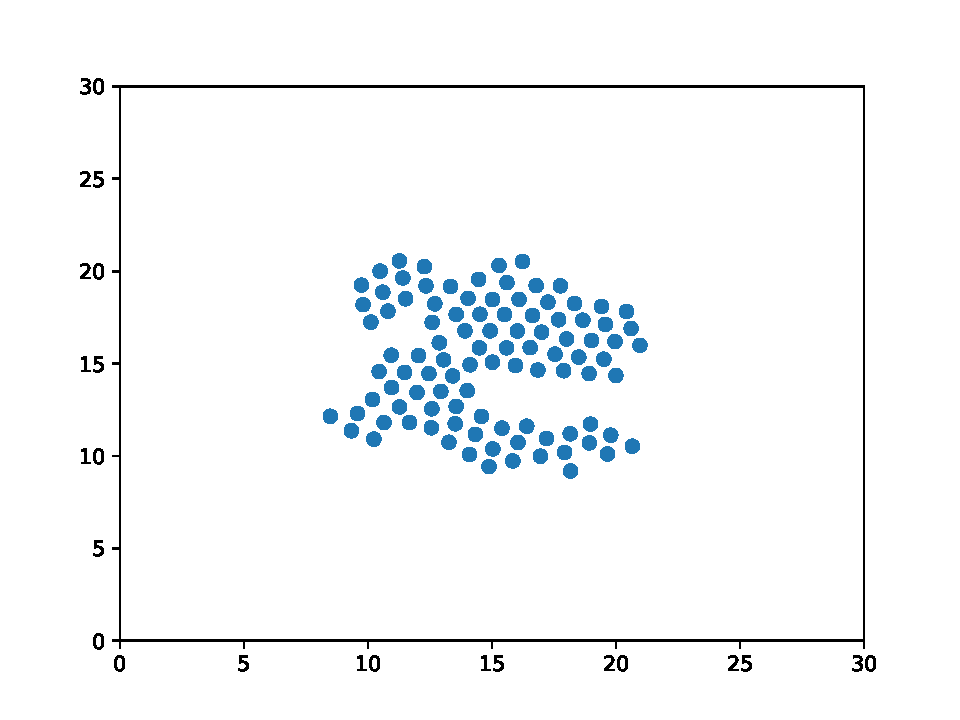
\includegraphics[width=0.5\linewidth]{writeup_plots/T10_start.pdf}}
  \subfloat{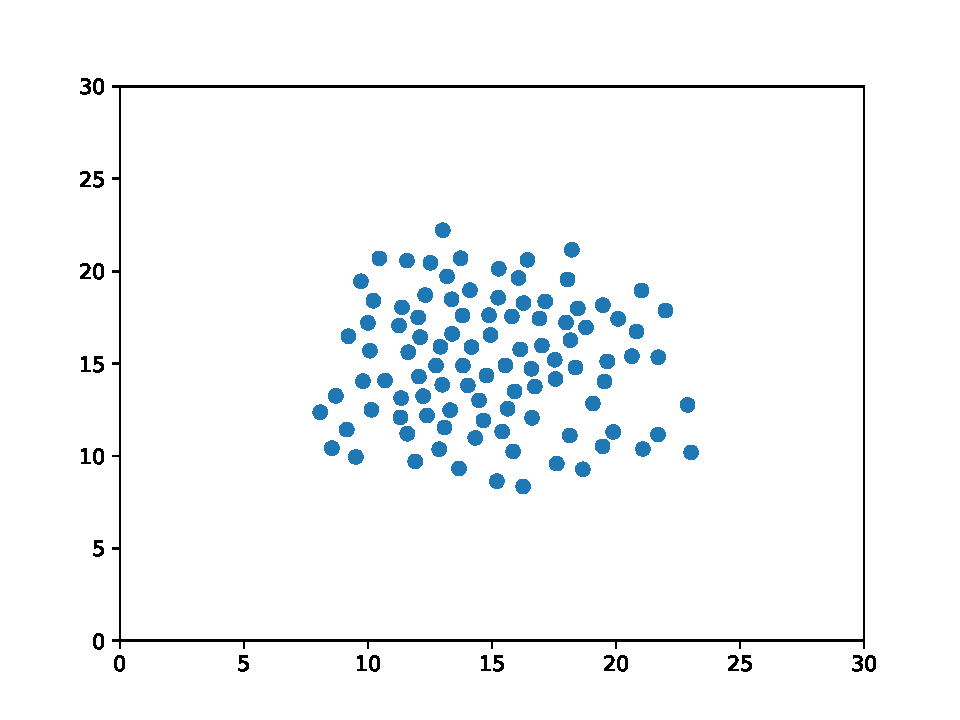
\includegraphics[width=0.5\linewidth]{writeup_plots/T10_end.pdf}}
  \caption{(Left to right) starting and ending configuration after $10000$
    timesteps of $h = 1e-3$.}
\end{figure}

\subsection{Gas}

The gas simulation was run by evolving from the initial conditions with a
temperature of $100$.

To view as an animation, run

\begin{minted}{bash}
python visualize.py 100
\end{minted}

The frames for the animated gif (see github) were created using the command:

\begin{minted}{bash}
python visualize.py 100 movie temp100 1000
\end{minted}

\begin{figure}[H]
  \subfloat{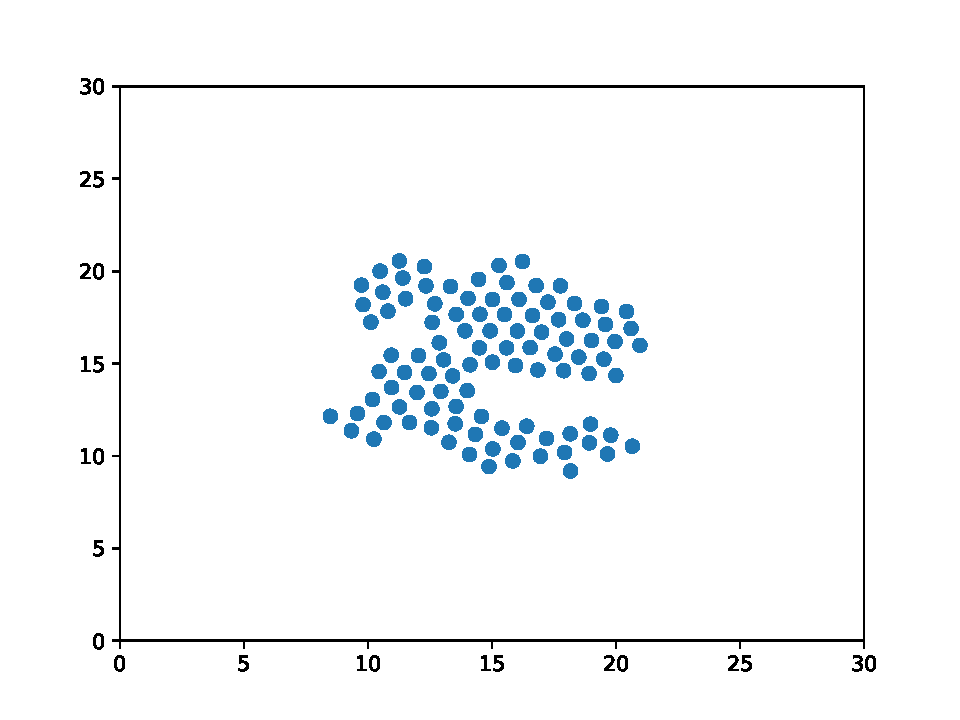
\includegraphics[width=0.5\linewidth]{writeup_plots/T100_start.pdf}}
  \subfloat{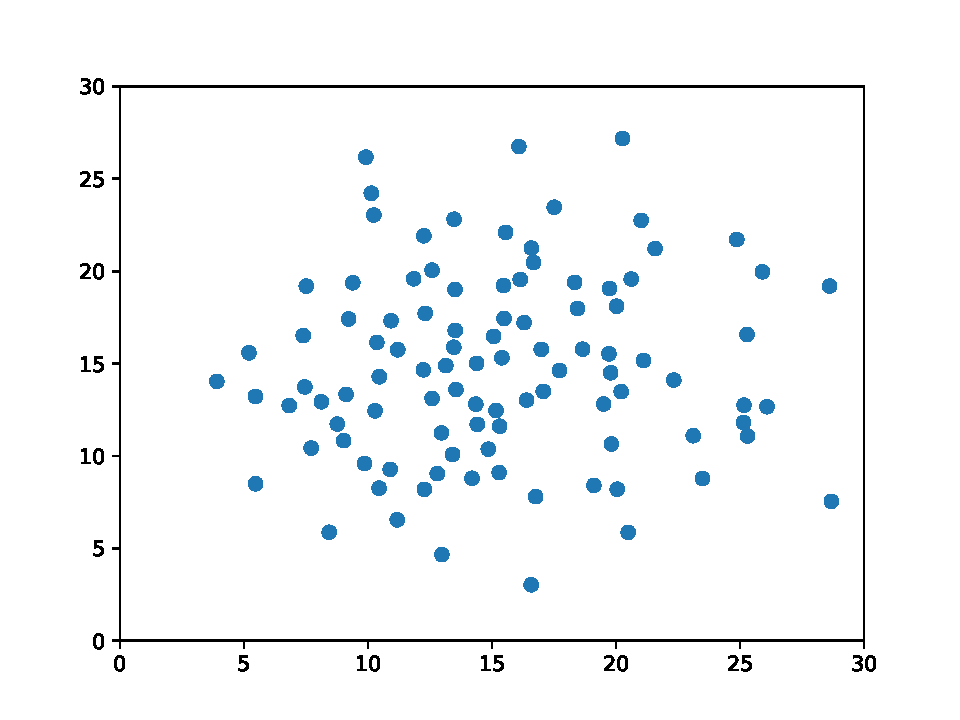
\includegraphics[width=0.5\linewidth]{writeup_plots/T100_end.pdf}}
  \caption{(Left to right) starting and ending configuration after $10000$
    timesteps of $h = 1e-3$.}
\end{figure}

\section*{Appendix}

\subsection*{Source Code}

\subsubsection*{molec.hpp}

\inputminted{c++}{molec.hpp}

\newpage

\subsubsection*{Molec.py}

\inputminted{python}{Molec.py}

\newpage

\subsubsection*{visualize.py}

\end{document}
